\documentclass[../main.tex]{subfiles}
\graphicspath{{\subfix{../../plots/daily_mean_temperature/}}}
\begin{document}
\section{Task 3.2}

For this task we analysed the mean temperature on each calendar year, across all years when the measurements were taken. As an example station Falsterbo was chosen. The result can be seen in figure~\ref{fig:placeholder}. \begin{figure}[H]
    \centering
    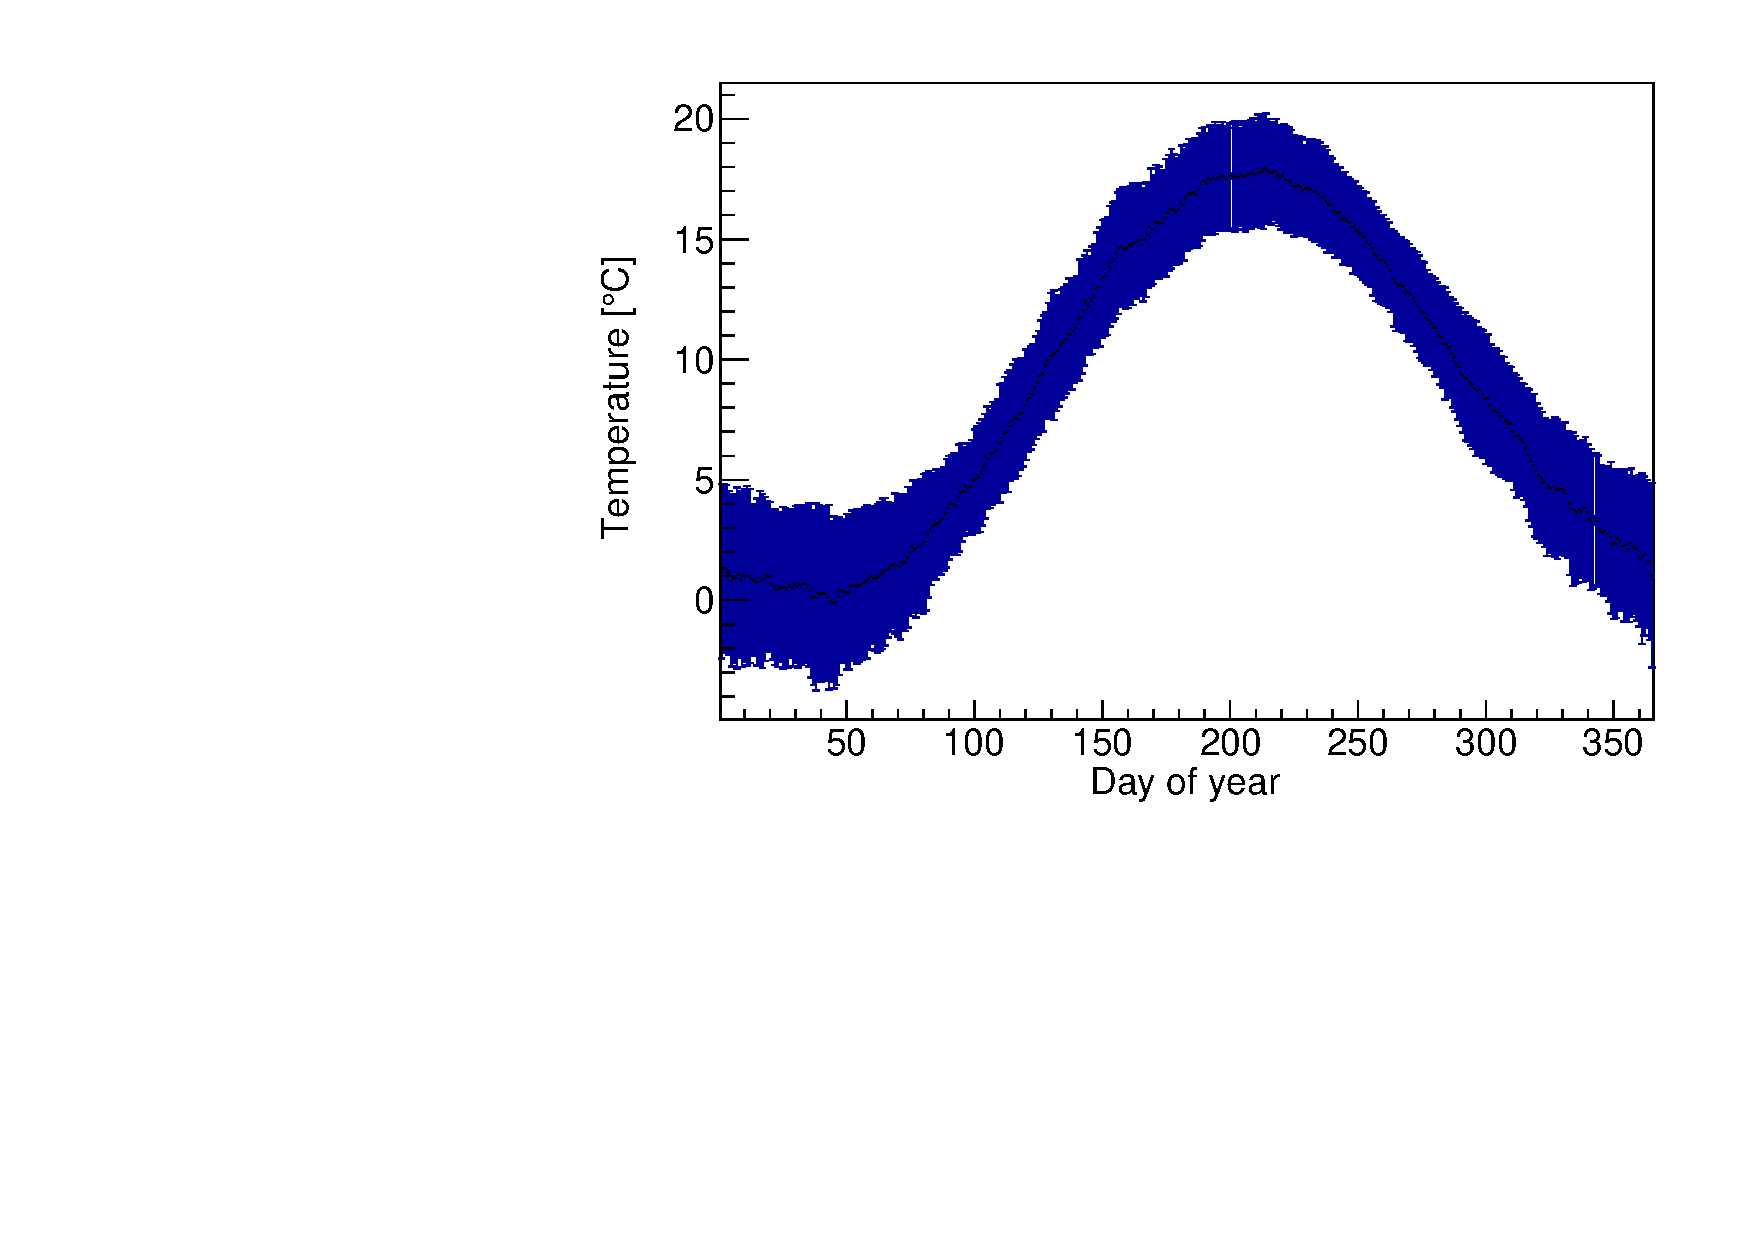
\includegraphics[width=1\linewidth]{daily_mean_over_years.pdf}
    \caption{Mean temperature for each calendar day over the years, Falsterbo.}
    \label{fig:placeholder}
\end{figure}
The initial approach I had for this task was to iterate through months, days and years and find tree entries that matched criteria. This approach did not work as the for loops were causing ROOT to crash, most likely as there were too many entries to go through. I have therefore decided to first select the measurements fitting the criteria (belonging to a chosen weather station). February 29 was excluded for convenience. \\

First, all selected entries were iterated through and their year and day indices were established. The corresponding temperature was added to an array of temperature sums for each day, while the counts for given day were counted in a separate array. In a separate loop each day index was iterated through for each year, and the means were found for all calendar days across the years. The means for each calendar day were summed, divided by the number of entries and added to the vector for final values, along with standard deviations calculated using ROOT's \verb|TMath::RMS|. The results were then plotted using \verb|TH1D| and displayed using \verb|TCanvas|.
\end{document}
